\documentclass{article}
\usepackage[utf8]{inputenc}
\usepackage[T1]{fontenc}
\usepackage{graphicx}
\usepackage{hyperref}
\usepackage{geometry}
\geometry{margin=1in}

\title{OPTICS and REFRACTION INSTRUMENTS (Plate XVII)}
\date{Encyclopaedia Britannica (1771)}

\begin{document}
\maketitle

\section*{Historical source}
\textbf{Entry ID:} \texttt{entry-britannica-volume-193819043-row-1845-1845} \\
\textbf{Volume ID:} 193819043 \\
\textbf{Character Count:} 706

\subsection*{Extracted Text}
XVII.

[HISTORICAL COPPERPLATE ENGRAVING: OPTICS and REFRACTION INSTRUMENTS (Plate XVII)]
Category: Physical Optics and Astronomy
Visual Description: Engraved copperplate illustrating optical refraction, ray tracing through convex and concave lenses, Newtonian prisms, and Gregorian/Newtonian reflecting telescope mirror configurations.
Identified Engraved Figures:
  * Fig. 1: Prismatic refraction and light dispersion into spectrum
  * Fig. 2: Compound achromatic lens system correcting chromatic aberration
  * Fig. 3: Reflecting telescope optical diagram with primary paraboloid mirror
Related Scientific Subjects: Optics, Refracting telescope, Dispersion (optics), Prism (optics), Reflecting telescope

\subsection*{Matched Wikipedia Article}
\textbf{Title:} History of the Encyclopædia Britannica \\
\textbf{Page ID:} 9004976 \\
\textbf{Revision ID:} 1340071003 \\
\textbf{URL:} \url{https://en.wikipedia.org/wiki/History\_of\_the\_Encyclop\%C3\%A6dia\_Britannica}


\section*{Source record}
\begin{itemize}
\item \textbf{Dataset:} \texttt{NationalLibraryOfScotland/encyclopaedia\_britannica\_illustrated}
\item \textbf{Dataset Revision:} \texttt{309f765b1ecc83e0a7f7762e44b4a927a7555443}
\item \textbf{Page ID:} \texttt{britannica:309f765b1ecc83e0a7f7762e44b4a927a7555443:train:1845} \\
  \textbf{Filename:} \texttt{page-1845-a758ad9d45a7.jpg} \\
  \textbf{Row Index:} 1845 \\
  \textbf{SHA256:} \texttt{a758ad9d45a7173d...}
\end{itemize}

\begin{figure}[h]
\centering
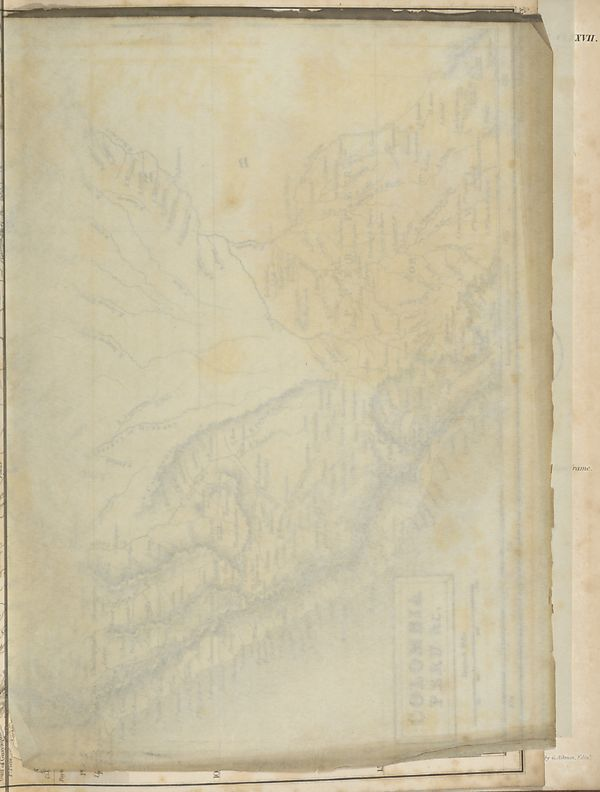
\includegraphics[width=0.85\textwidth]{../scans/page-1845-a758ad9d45a7.jpg}
\caption*{Source scan: \texttt{page-1845-a758ad9d45a7.jpg}}
\end{figure}

\end{document}
